\documentclass[../../main.tex]{subfiles}
\begin{document}

\subsection*{10.2}
Una spira conduttrice quadrata, di lato $b = 20\ cm$, massa $m = 4\ g$, resistenza $R = 25\ \Omega$, si muove senza attrito sul piano x,y con velocità costante $v_0 = 4 * 10^{-2}\ \frac{m}{s}$. Per $x\ge0$ esiste un campo magnetico uniforme e costante di valore $B = 0.5\ T$ e la spira entra in questa regione all'istante t = 0.\\
Calcolare la velocità $v_1$ raggiunta dalla spira dopo $t_1 = 2.9\ s$ sapendo che in quell'istante la spira è ancora soltanto parzialmente inserita nel campo, l'energia dissipata nel circuito fino al tempo $t_1$, la velocità $v_2$, la carica $q$ che circola nella spira durante l'intero processo.\\
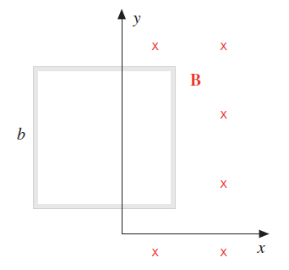
\includegraphics[scale=0.3]{e_10_2.png}
\subsubsection*{Formule utilizzate}
$\vec{E_i} = \frac{\vec{F}}{q} = \vec{v}\wedge\vec{B}$\\
$\varepsilon_i = vBb$\\
$i = \frac{vbB}{R}$
\subsubsection*{Soluzione punto a}
La forza sul lato destro in movimento del circuito vale:\\
$F =i b B = \frac{vb^2B^2}{R}$ opposta al moto.\\
Il modo diventa $m\frac{dv}{dt}=-\frac{vb^2B^2}{R}$\\
$log\frac{v(t)}{v_0}=-\frac{b^2B^2}{mR}t$\\
Il moto risulta esponenzialmente smorzato\\
$v(t) = v_0\ exp(-\frac{t}{\tau})$\\
Con costante di tempo: $\tau = \frac{mR}{b^2B^2} = 10\ s$\\
$v_1 = v_0\ exp(-\frac{t_1}{\tau}) = 3 * 10^{-2}\ \frac{m}{s}$\\
Il lavoro si trova come variazione di energia cinetica della barra\\
$W = \frac{1}{2}m\left(v_0^2-v_1^2\right) = 1.4 * 10^{-6}\ J$\\
Questa energia è stata dissipata in effeto Joule. Infatti:\\
$i = \frac{m}{bB}\frac{dv}{dt} = \frac{m}{bB}\frac{v_0}{\tau}\ exp\left(-\frac{t}{\tau}\right) = \frac{v_0}{R}bB\ exp\left(-\frac{t}{\tau}\right)$\\
da cui l'energia dissipata per effetto Joule è:\\
$W = \int_0^tRi^2dt = R\frac{v_0^2}{R^2}b^2B^2\int_0^te^{-\frac{2t}{\tau}} dt = \frac{v_0^2b^2B^2}{R}\frac{\tau}{2}\left[1- e^{-\frac{2t}{\tau}}\right] = \frac{1}{2}mv_0^2\left[1-e^{-\frac{2t}{\tau}}\right] = 1.4 * 10^{-6}\ J$\\
Esprimendo la velocità in funzione di x:\\
$\frac{dv}{dx} = \frac{dv}{dt}\frac{dt}{dx} = \frac{dv}{dt}\frac{1}{v} = -\frac{1}{\tau}$\\
Tale equazione integrata:\\
$v(x) = v_0 - \frac{x}{\tau}$\\
Quando la spira è totalmente entrata la velocità rimane costante e pari a:\\
$v_2 = v_0 - \frac{b}{\tau} = 2.10^{-2}\ \frac{m}{s}$\\
Usando l'espressione per v(t):\\
$v_2 = v_0\ exp\left(-\frac{t_2}{\tau}\right)$\tab$t_2 = \tau ln\left(\frac{v_0}{v_2}\right) = 6.9\ s$\\
\subsubsection*{Soluzione punto b}
Per calcolare la carica che che circola nella spira nell'intero processo si applica la legge di Felici:\\
$q = \frac{\Delta\Phi}{R} = \frac{Bb^2}{R} = 8 * 10 ^{-4}\ C$
\newpage

\end{document}